\scanpage{138}
\mspage{1}
\deleted{$a_{i0}$}
\[
\left\{\begin{array}{l}
f_i=a_i+\displaystyle\sum_{1\leq j\leq n}b_{ij}t_j+\displaystyle\sum_{|p|\geq2}c_{ip}t^p\\[-2pt]
\hspace{2em}\deleted{\unsure{\in\mathfrak m|0}}\\
1\leq i\leq n
\end{array}\right.
\qquad a_i,b_{ij},c_{ip}\in A
\qquad\left\{\begin{array}{l}a_i\in\mathfrak m\\ \det(b_{ij})\unsure{\notin|\in}\unsure{A\mathfrak m|A^\times}\end{array}\right.
\]
\diagram{\begin{tikzcd}[ampersand replacement=\&,column sep=huge]
(\lambda_1,\unsure{-|\ldots}\lambda_n)\in\mathfrak m^{(\times n)} \arrow[r,squiggly,"\lambda_{(f=(f_1,\unsure{-|\ldots} f_n))}"'] \& (f_1(\lambda_1,\unsure{-|\ldots},\lambda_n),\unsure{-|\ldots},f_n(\lambda_1,\unsure{-|\ldots}\lambda_n))
\end{tikzcd}}

Si $A$ est d'ordre infinitésimal $N$, alors $\lambda_f$ est connu quand on connaît $f\mod(t_1,\unsure{-|\ldots} t_n)^{N+1}$, donc \unsure{quand on} connaît \deleted{les} $\unsure{N|n}$ \uline{polynômes} en $t$ de degré $\leq N$.
\deleted{\unsure{ou}}
\[
\boxed{f_i(\lambda_1,\unsure{-|\ldots}\lambda_n)=a_i+\sum_jb_{ij}\lambda_j+\sum_{2\leq|p|\leq N}c_{ip}\lambda_1^{p_1}\unsure{-|\ldots}\lambda_n^{p_n}}
\]
\diagram{\begin{tikzcd}[ampersand replacement=\&]
B=A[[t_1,\unsure{-|\ldots} t_n]]\\
A\arrow[u]
\end{tikzcd}}
\figure{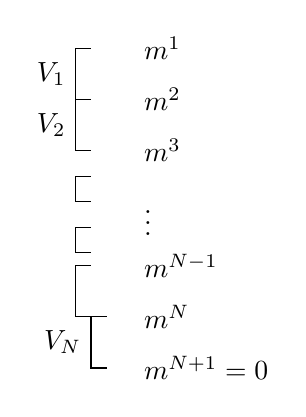
\begin{tikzpicture}[x=1cm,y=.65cm]
\node[anchor=west] at (1,0) {$\mathfrak m^{\deleted{\unsure{1}}}$};
\node[anchor=west] at (1,-1) {$\mathfrak m^2$};
\node[anchor=west] at (1,-2) {$\mathfrak m^3$};
\node[anchor=west] at (1,-3.25) {$\vdots$};
\node[anchor=west] at (1,-4.25) {$\mathfrak m^{N-1}$};
\node[anchor=west] at (1,-5.25) {$\mathfrak m^N$};
\node[anchor=west] at (1,-6.25) {$\mathfrak m^{N+1}=0$};
\draw (.45,0)--(.25,0)--(.25,-1)--(.45,-1);
\draw (.45,-1)--(.25,-1)--(.25,-2)--(.45,-2);
\draw (.45,-2.5)--(.25,-2.5)--(.25,-3)--(.45,-3);
\draw (.45,-3.5)--(.25,-3.5)--(.25,-4)--(.45,-4);
\draw (.45,-4.25)--(.25,-4.25)--(.25,-5.25)--(.45,-5.25);
\draw (.65,-5.25)--(.45,-5.25)--(.45,-6.25)--(.65,-6.25);
\node[left] at (.25,-.5) {$V_1$};\node[left] at (.25,-1.5) {$V_2$};\node[left] at (.45,-5.75) {$V_N$};
\end{tikzpicture}}
\margin{137}
